\paragraph{Sơ đồ quan hệ thực thể}
\mbox{}\par

ERD gồm 11 thực thể, chia thành các nhóm tài khoản, quan hệ bạn bè,
hội thoại và tin nhắn, báo cáo spam, đăng nhập và hoạt động.
\texttt{Conversation} được dùng chung cho hội thoại riêng và nhóm chat,
phân biệt bằng thuộc tính \texttt{type}. Thành viên và quyền trong từng
hội thoại được quản lý qua \texttt{ConversationMember}.

Hình~\ref{fig:erd-chatapp-v1} trình bày toàn bộ mô hình. Các thuộc tính
được mô tả lại trong Bảng~\ref{tab:tu-dien-du-lieu} để thuận tiện tra cứu.
Trong hình, PK là khóa chính, FK là khóa ngoại, UK là giá trị duy nhất;
dấu hỏi biểu thị thuộc tính có thể chưa có giá trị. Ký hiệu 1 và 0..N
thể hiện quan hệ một--nhiều, trong đó phía nhiều có thể chưa có bản ghi.

\begin{landscape}
\begin{figure}[p]
  \centering
  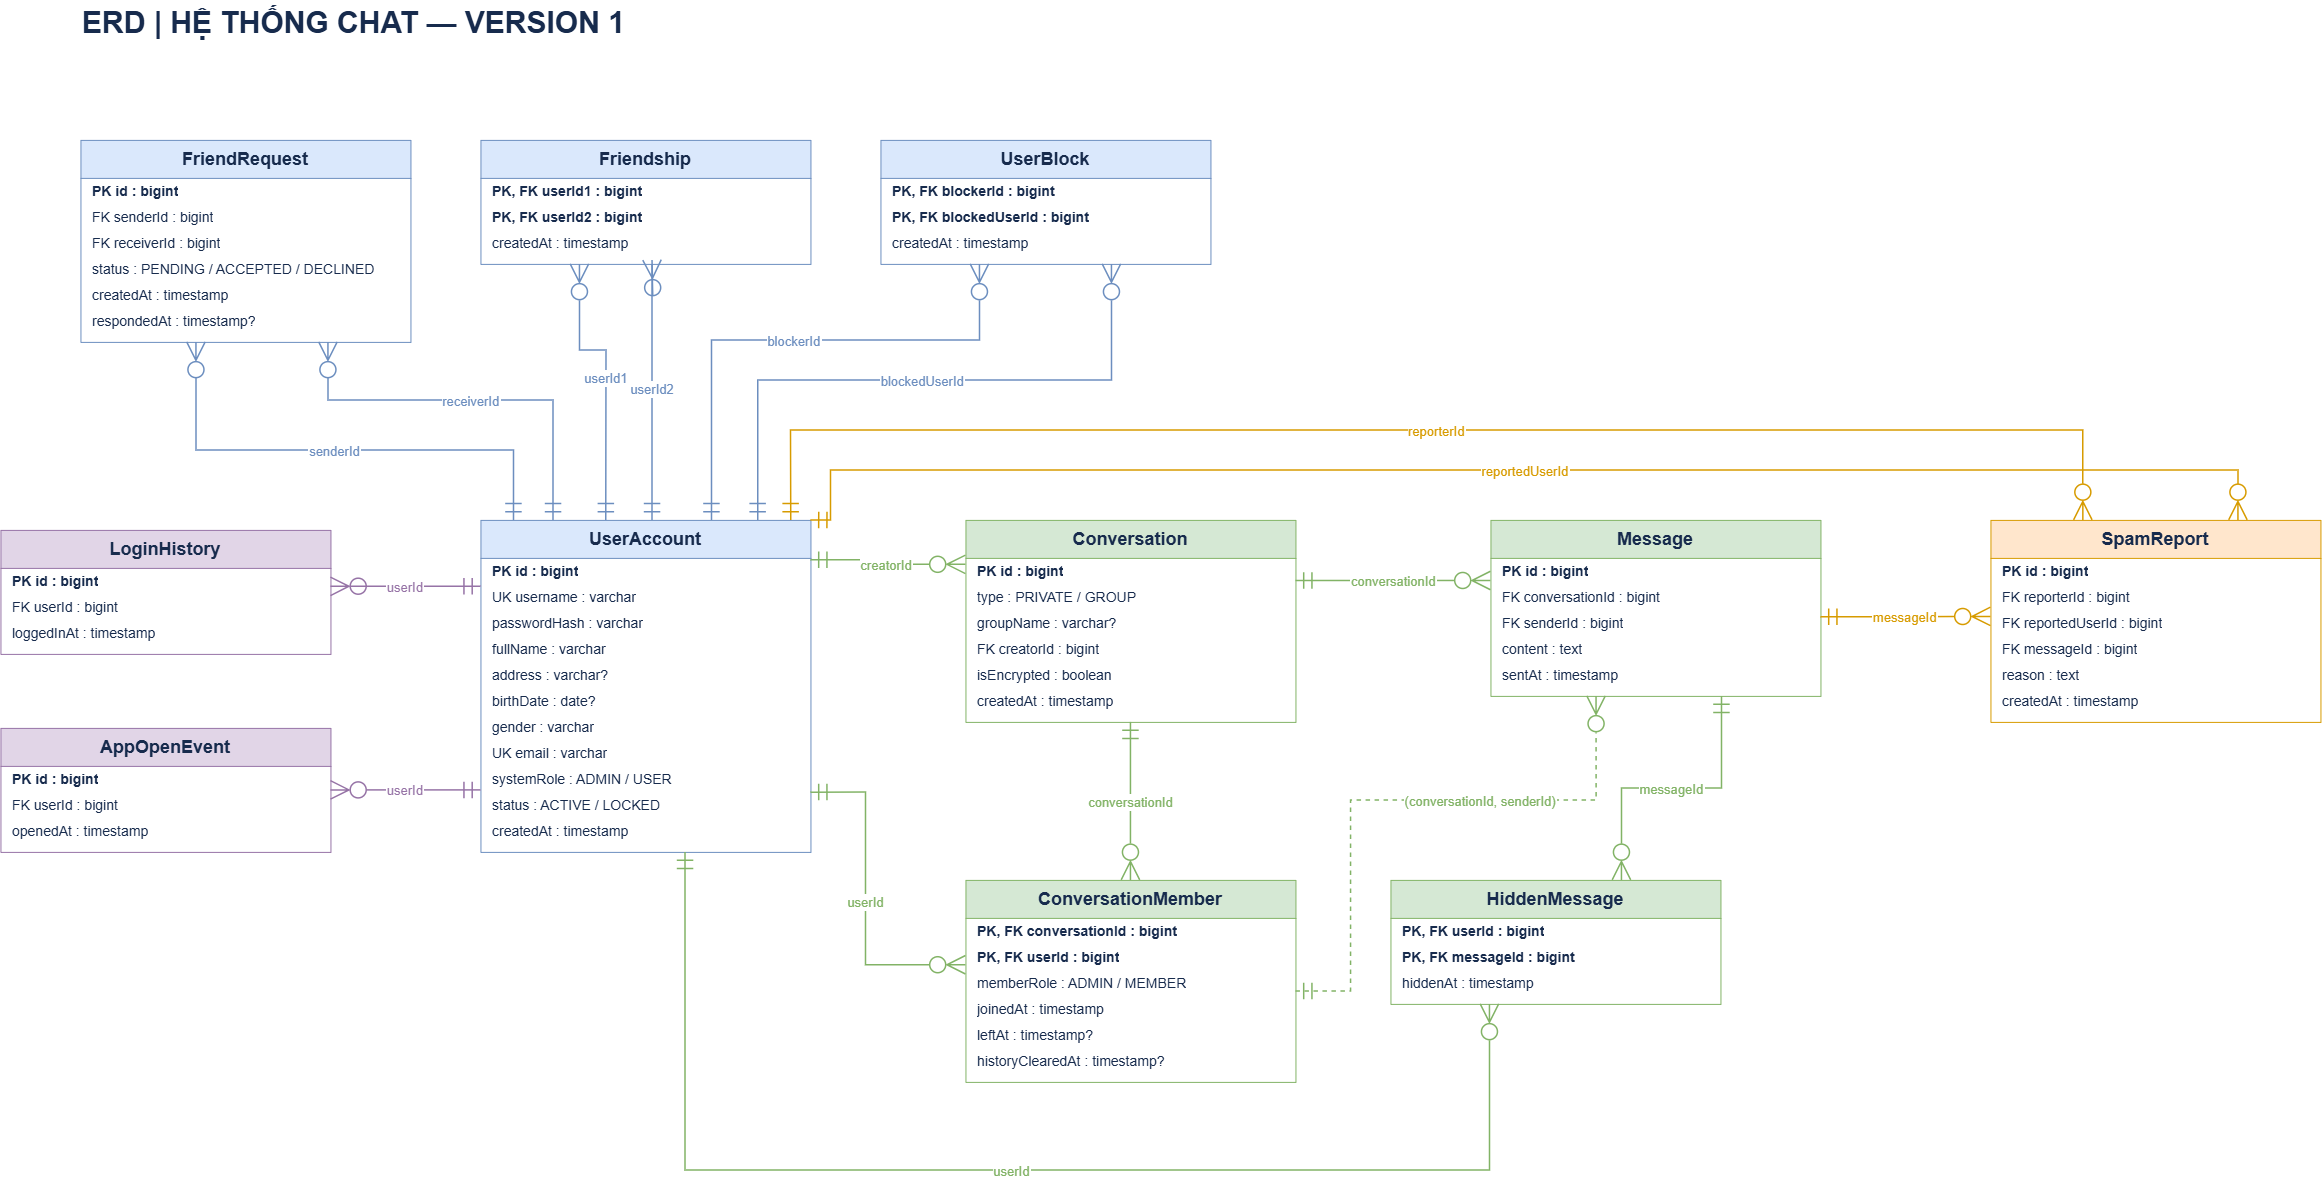
\includegraphics[width=\linewidth,height=0.83\textheight,keepaspectratio]{images/ERD-chatapp-v1.drawio.png}
  \caption{Sơ đồ quan hệ thực thể của hệ thống chat.}
  \label{fig:erd-chatapp-v1}
\end{figure}
\end{landscape}

Tên thực thể và tên thuộc tính trong phần mô tả được giữ thống nhất với
sơ đồ. Kiểu dữ liệu trong ERD được thể hiện ở mức logic; độ dài chuỗi,
giá trị mặc định và chính sách xử lý khi xóa dữ liệu cần được chốt khi
hoàn thiện script PostgreSQL.
